
\documentclass{article}
\usepackage[utf8]{inputenc}

\title{Laboratorio04_CALIDAD_PRUEBAS_SOFTWARE}
\author{edwartbalcon }
\date{October 2020}

\usepackage[utf8]{inputenc}
\usepackage[spanish]{babel}
\usepackage{natbib}
\usepackage{graphicx}

\begin{document}

\title{Caratula}

\begin{titlepage}
\begin{center}
\begin{Large}
\textbf{UNIVERSIDAD PRIVADA DE TACNA} \\
\end{Large}
\vspace*{-0.025in}
\begin{figure}[htb]
\begin{center}

\includegraphics[width=6cm]{./images/logo_UPT}
\end{center}
\end{figure}
\vspace*{-0.025in}
\begin{Large}
\textbf{FACULTAD DE INGENIERIA} \\
\end{Large}
\vspace*{0.05in}
\begin{Large}
\textbf{Escuela Profesional de Ingeniería de Sistema} \\
\end{Large}


\vspace*{0.4in}

\vspace*{0.1in}
\begin{Large}
\textbf{Informe de laboratorio 02: Crear y consultar una tabla NoSQL} \\
\end{Large}

\vspace*{0.3in}
\begin{Large}
\textbf{Curso: Base de datos II} \\
\end{Large}

\vspace*{0.3in}
\begin{Large}
\textbf{DOCENTE: Ing. Patrick Cuadros Quiroga} \\
\end{Large}

\vspace*{0.2in}
\vspace*{0.1in}
\begin{large}

\begin{Large}
\textbf{Alumno: Balcon Coahila, Edwart Juan\hfill	(2013046516) } \\
\end{Large}

\vspace*{0.15in}
\begin{Large}
\textbf{Tacna – Perú} \\
\end{Large}

\vspace*{0.05in}
\begin{Large}
\textbf{2020 } \\
\end{Large}

\end{large}
\end{center}

\end{titlepage}


\newpage

\section{ Creación de una tabla NoSQL}

\textbf{1.1. En la consola de DynamoDB, haga clic en Create table.}

    \begin{center}
		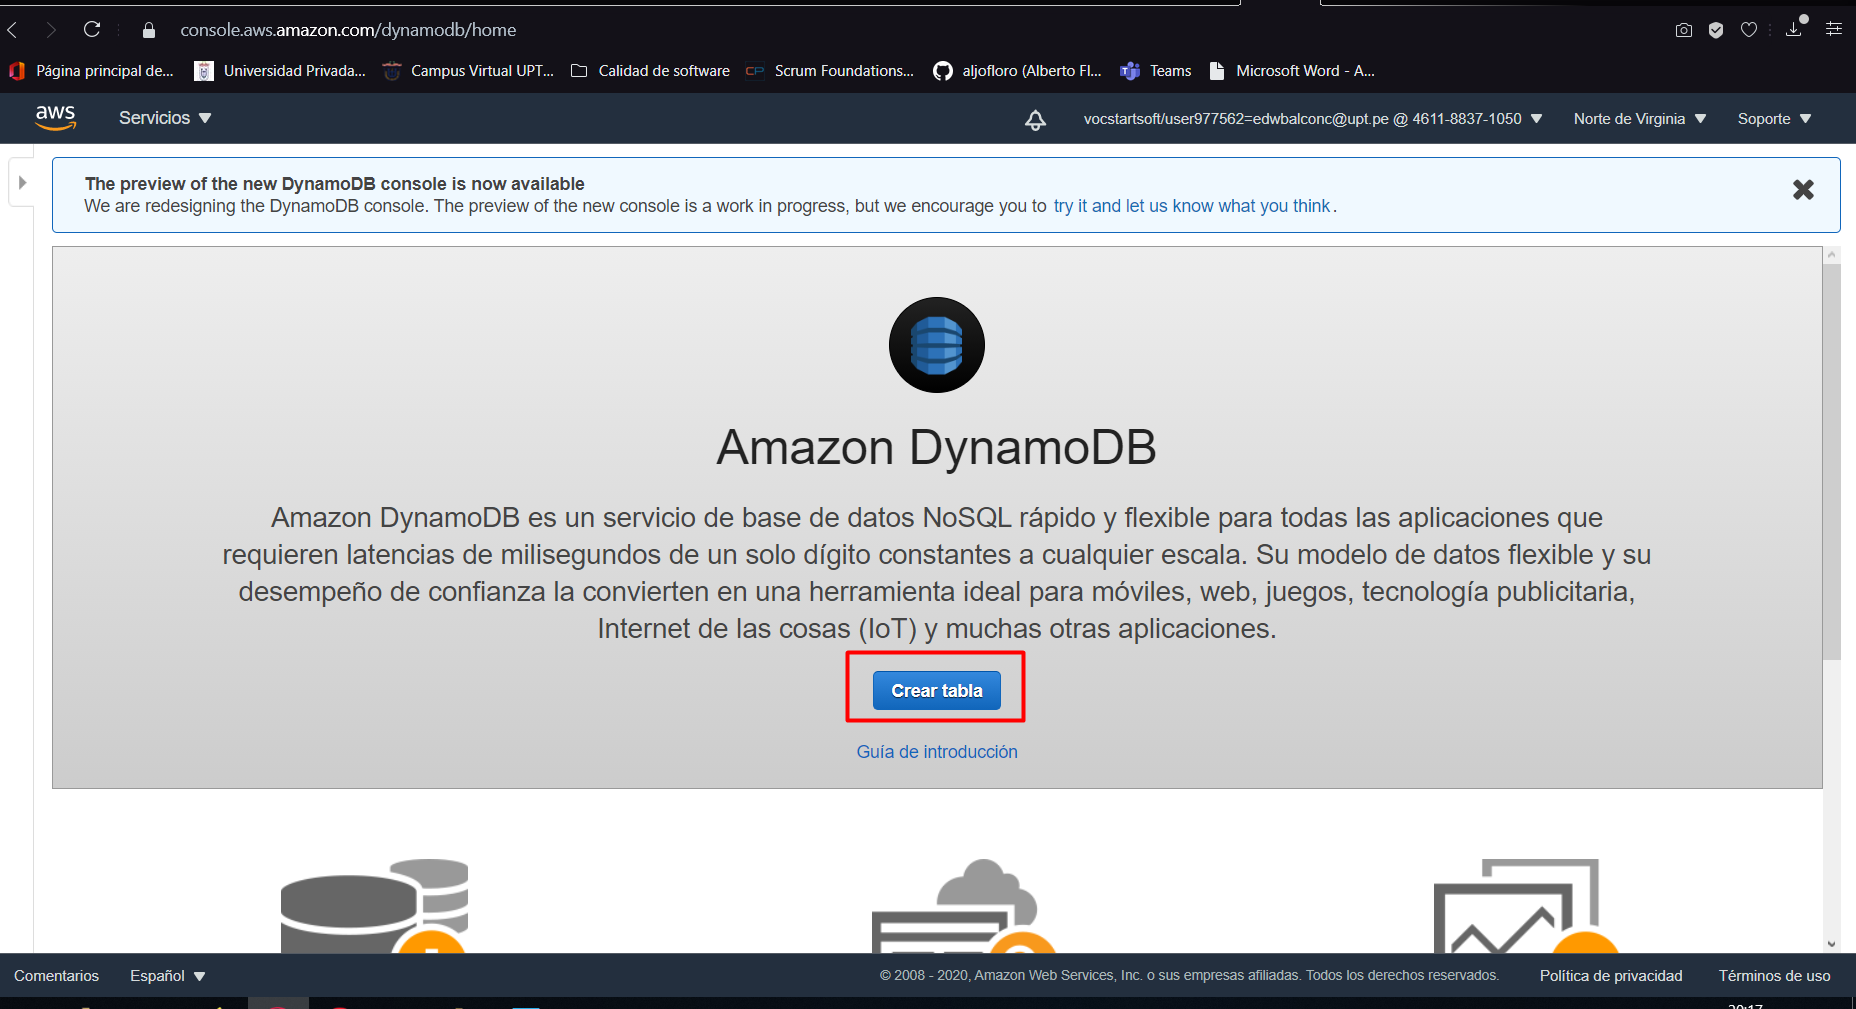
\includegraphics[width=15cm]{./images/1} 
	\end{center}
	\newpage
\textbf{1.2.Utilizaremos una biblioteca de música como nuestro caso de uso.  En el campo Table name (Nombre de la tabla), escriba Music.}

    \begin{center}
		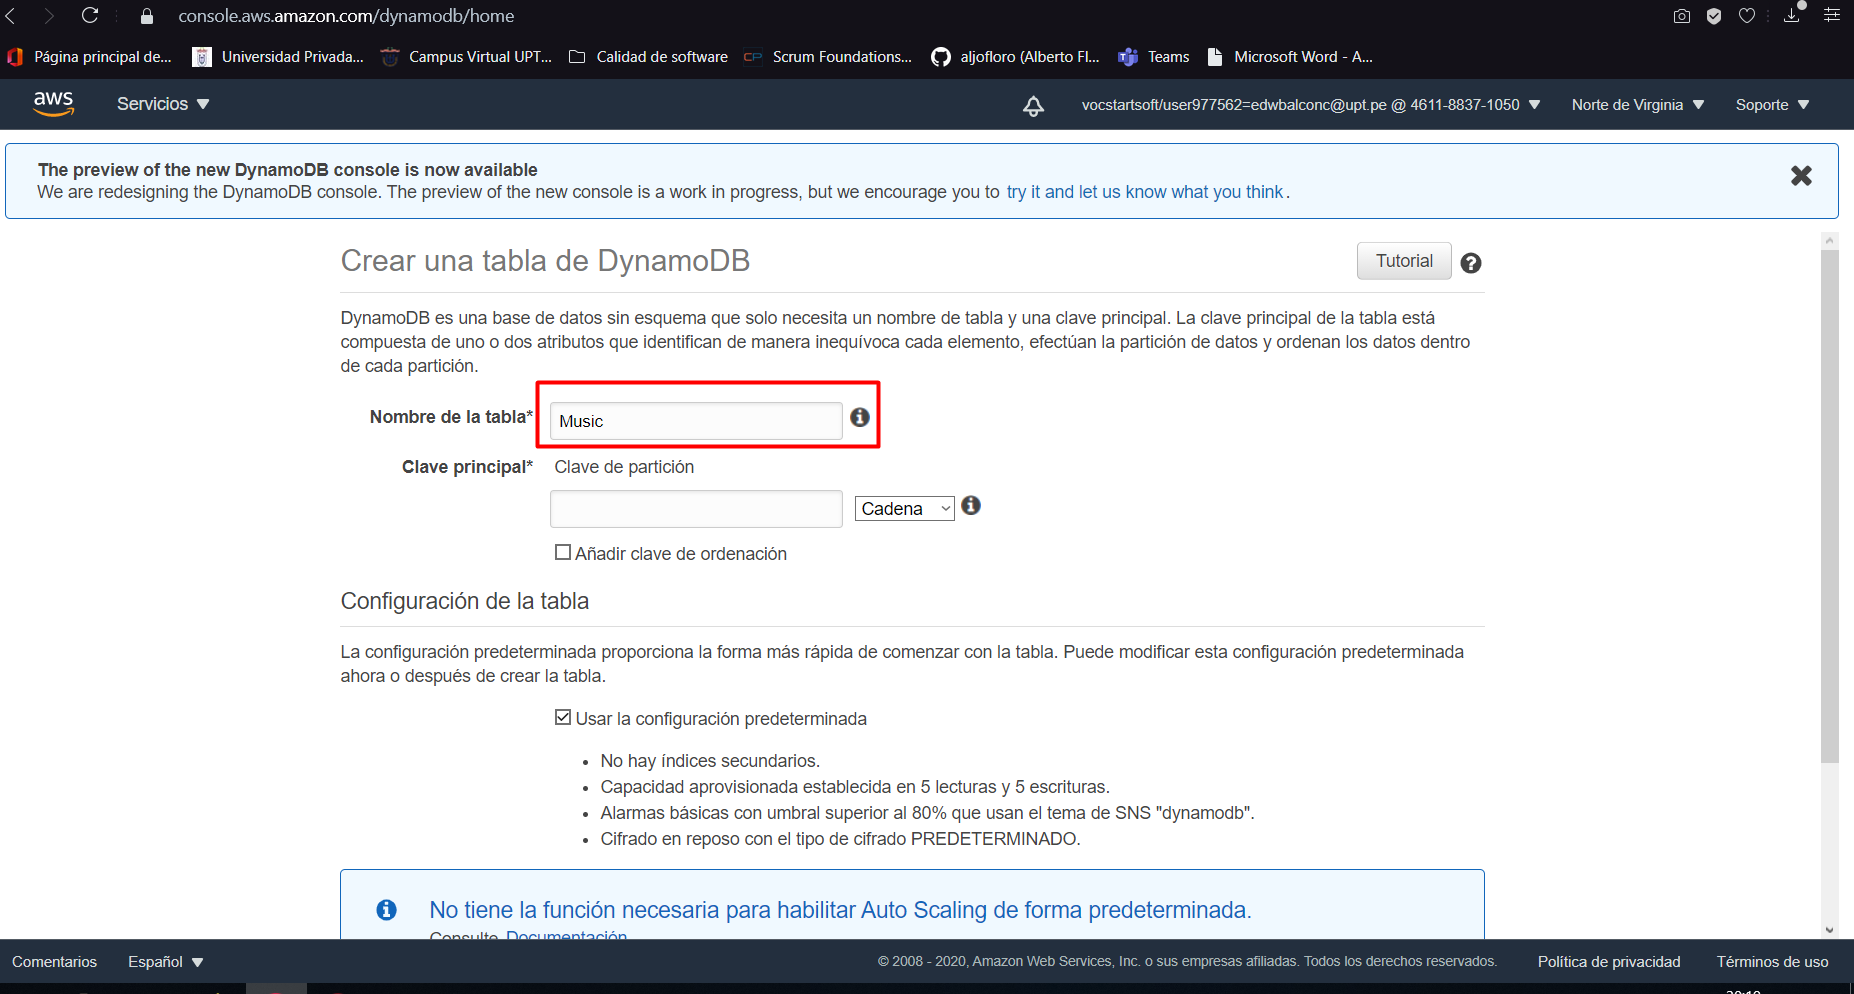
\includegraphics[width=15cm]{./images/2} 
	\end{center}
\newpage
\textbf{1.3. La clave de partición se utiliza para repartir datos por las particiones con fines de escalabilidad. Es importante elegir un atributo con una amplia gama de valores y que es probable que tenga patrones de acceso de distribución uniforme. Escriba Artist en el campo Partition Key (Clave de partición).
}

    \begin{center}
		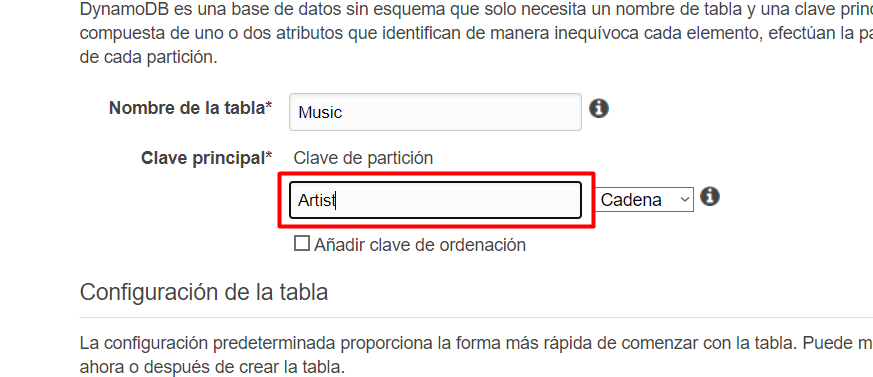
\includegraphics[width=15cm]{./images/3} 
	\end{center}


\textbf{1.4. Dado que cada artista puede componer muchas canciones, puede habilitar el ordenamiento sencillo con una clave de ordenamiento. Marque la casilla Add sort key (Añadir clave de ordenamiento). Escriba songTitle en el campo Add sort key (Añadir clave de ordenamiento). }

    \begin{center}
		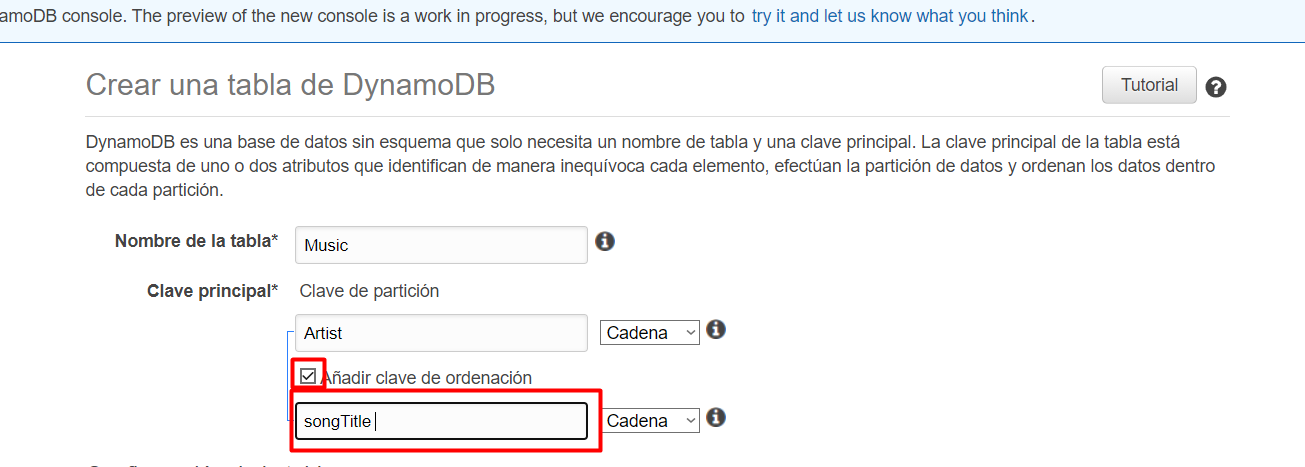
\includegraphics[width=15cm]{./images/4} 
	\end{center}
	\newpage
\textbf{1.5. A continuación, activaremos DynamoDB Auto Scaling para nuestra tabla.
}

    \begin{center}
		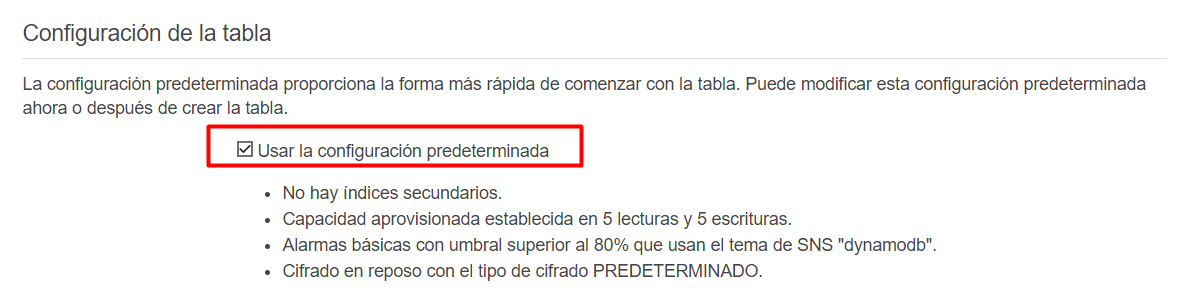
\includegraphics[width=15cm]{./images/5} 
	\end{center}
\textbf{1.6.Desplácese hacia la parte inferior de la pantalla, pasando Secondary indexes (Índices secundarios), Provisioned capacity (Capacidad aprovisionada) y Auto Scaling hasta llegar al botón Create. 
}

    \begin{center}
		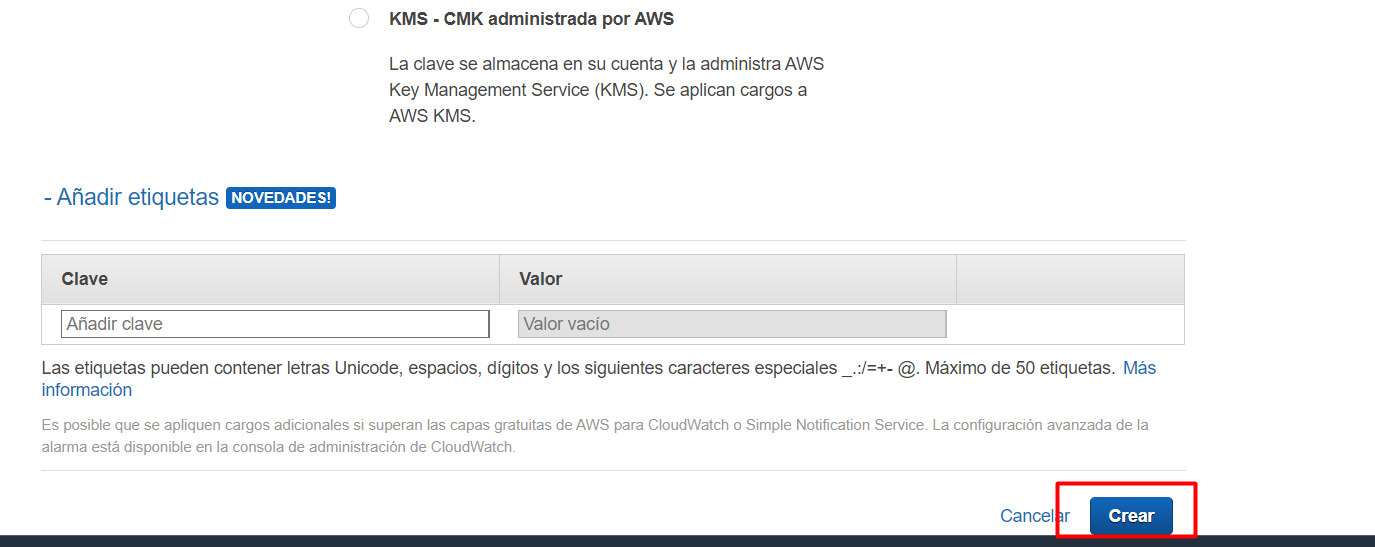
\includegraphics[width=15cm]{./images/6.} 
	\end{center}

\newpage

\section{Agregar datos a la tabla NoSQL }

\textbf{2.1. Haga clic en la pestaña Items (Elementos). Bajo la pestaña Items (Elementos), haga clic en Create item (Crear elemento) . }

    \begin{center}
		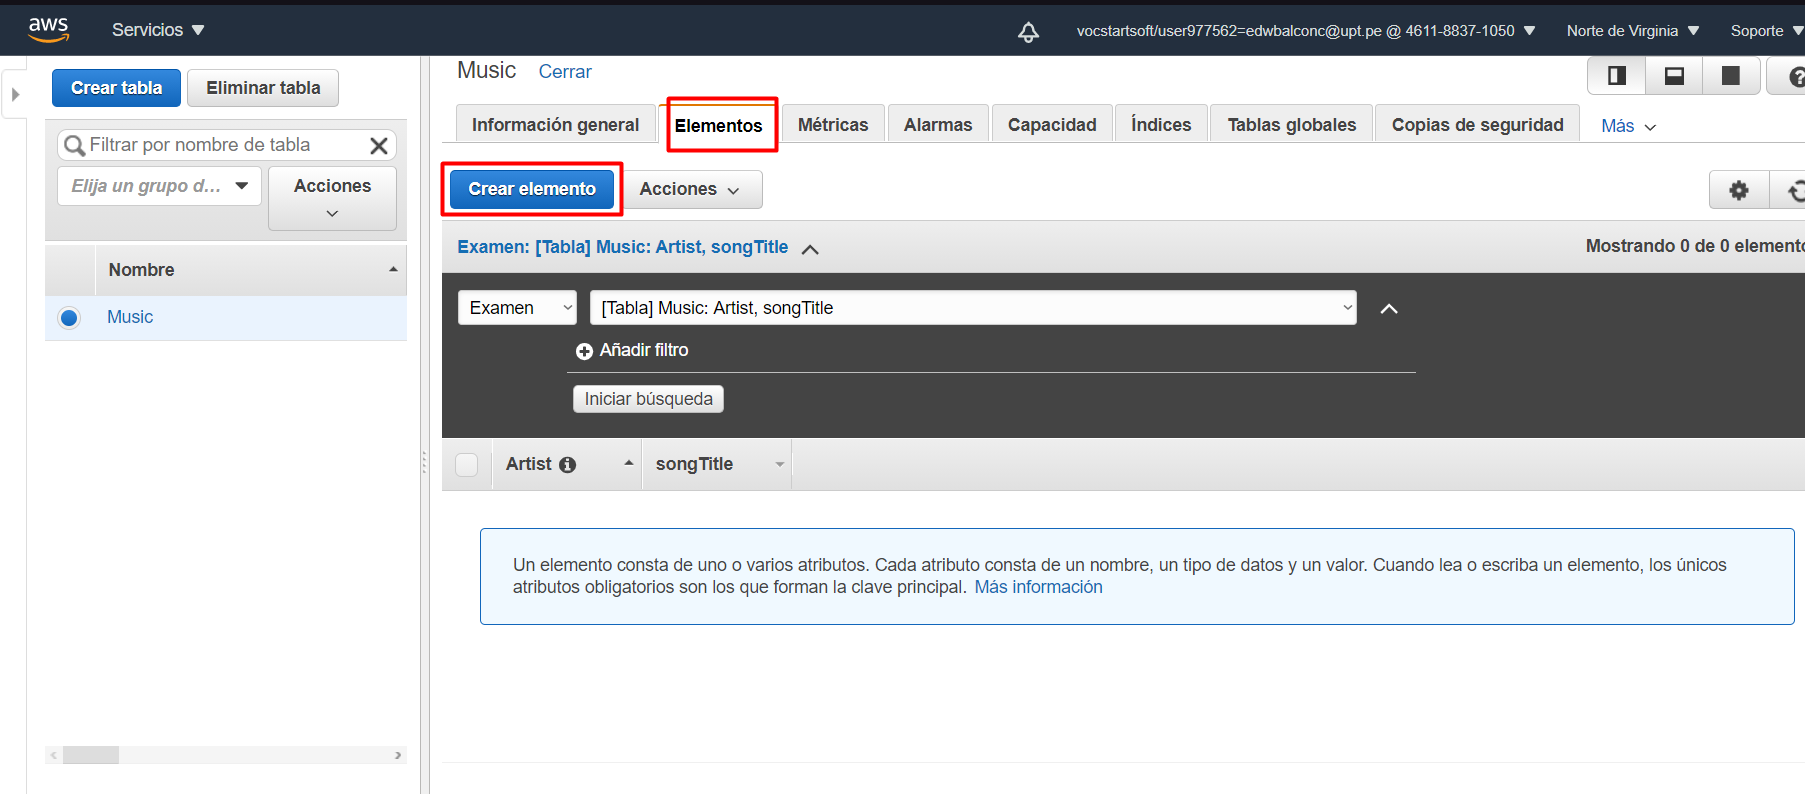
\includegraphics[width=15cm]{./images/7} 
	\end{center}
	\newpage
\textbf{2.2.En la ventana de introducción de datos, escriba lo siguiente: }

    \begin{center}
		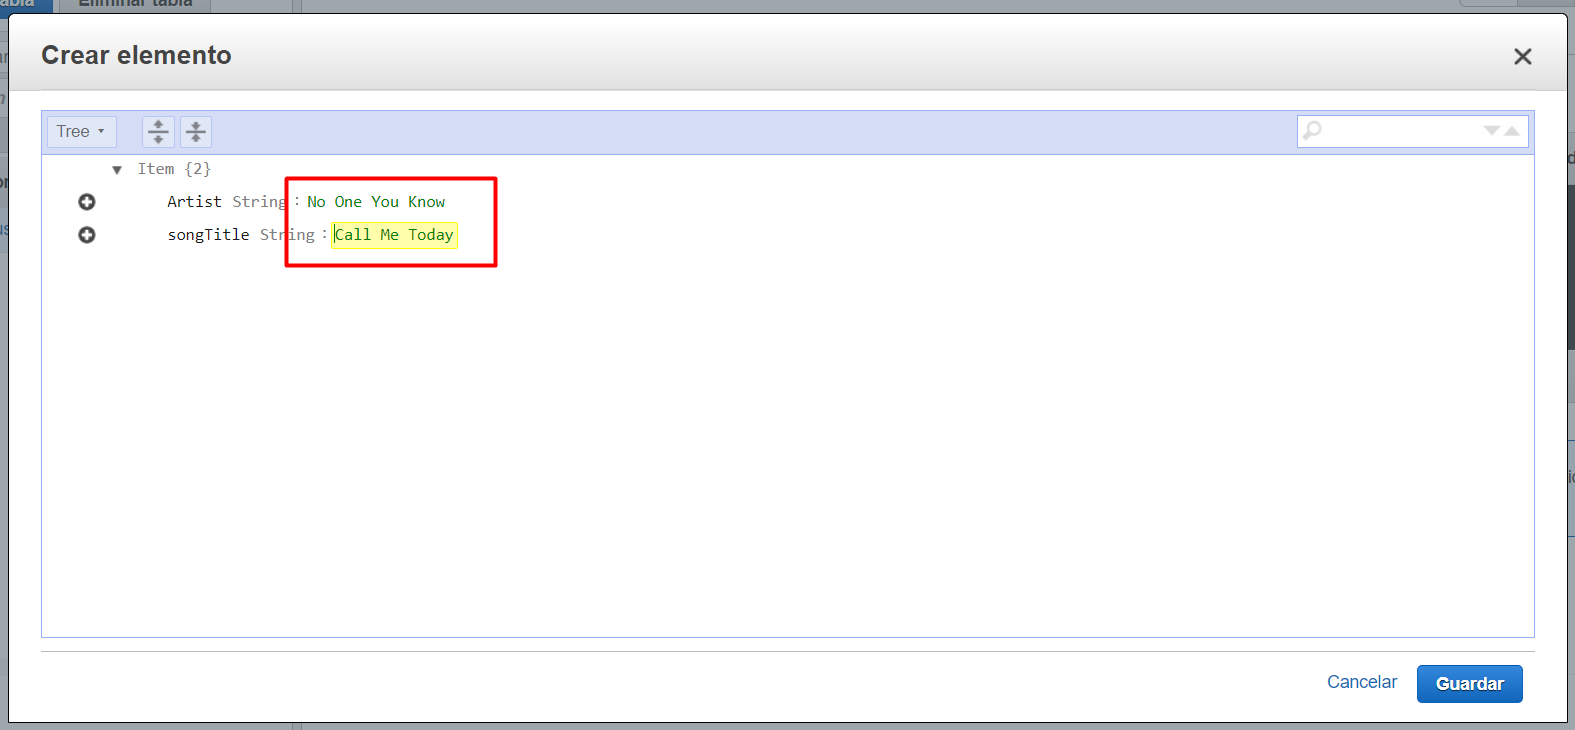
\includegraphics[width=15cm]{./images/8} 
	\end{center}
\textbf{2.3. Repita el proceso para agregar algunos elementos más a la tabla Music:
}
 \begin{center}
		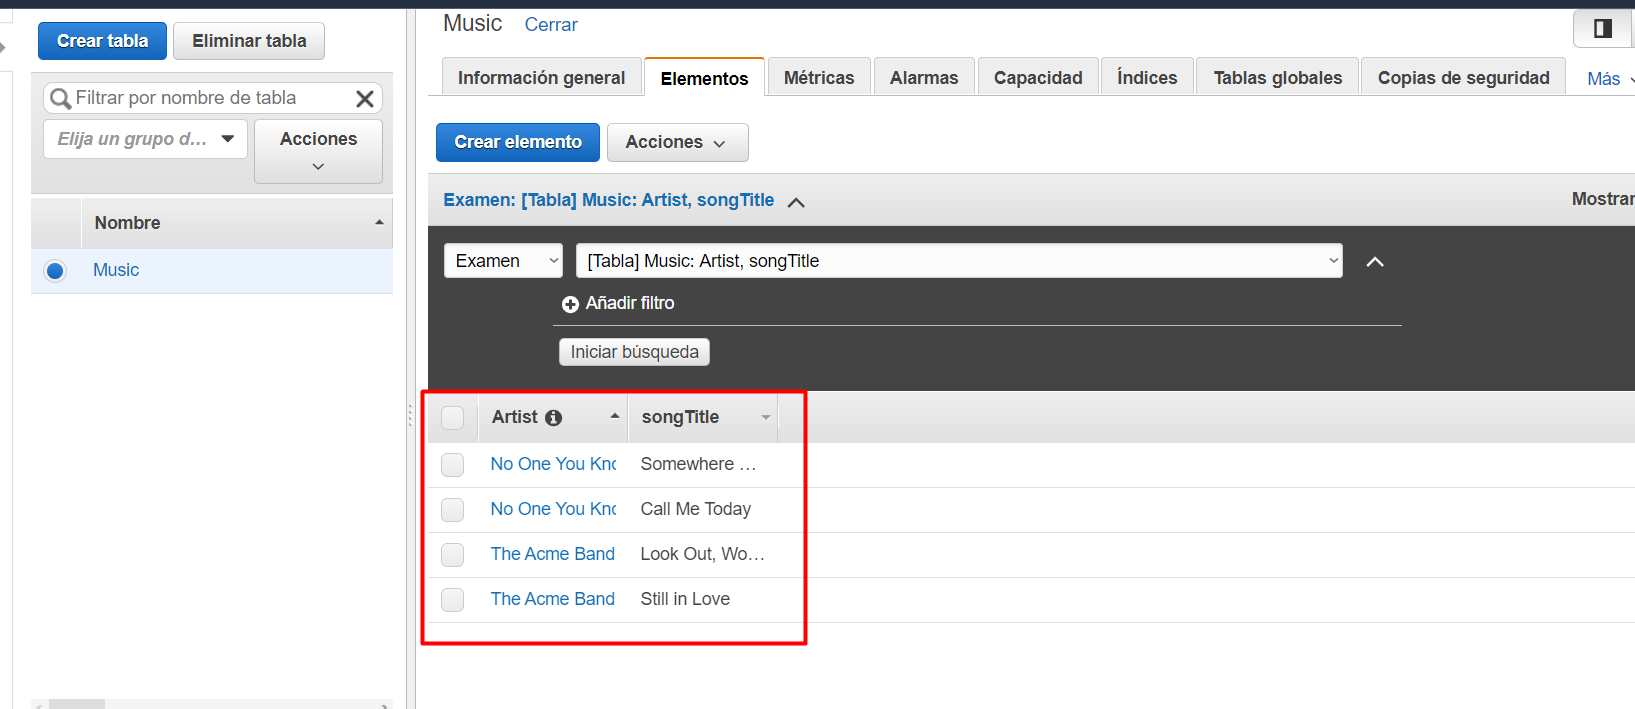
\includegraphics[width=15cm]{./images/9} 
	\end{center}
	
	\newpage

\section{Consulta de la tabla NoSQL }

\textbf{3.1. Mediante la lista desplegable situada en el banner gris oscuro encima de los elementos, cambie Scan (Escaneo) a Query (Consulta). }

    \begin{center}
		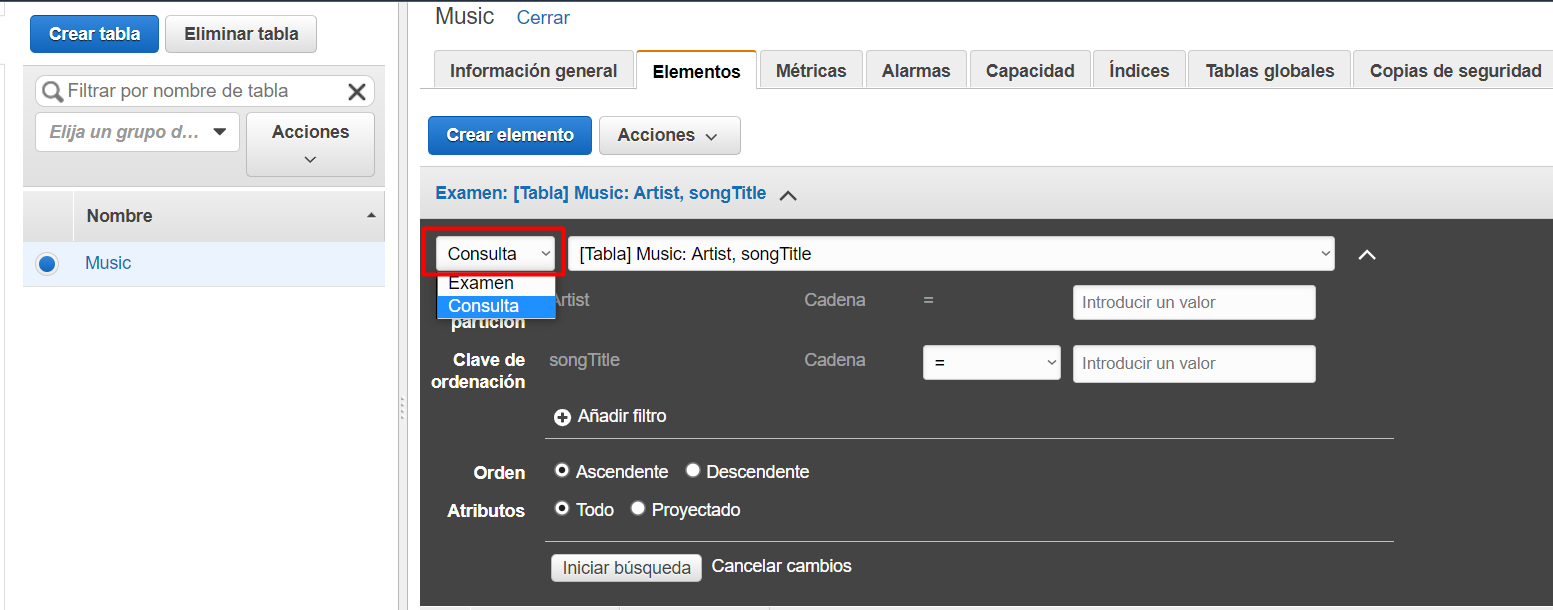
\includegraphics[width=15cm]{./images/10} 
	\end{center}
\textbf{3.2.Puede utilizar la consola para consultar la tabla Music de diversas formas. Para la primera consulta, realice lo siguiente: }

    \begin{center}
		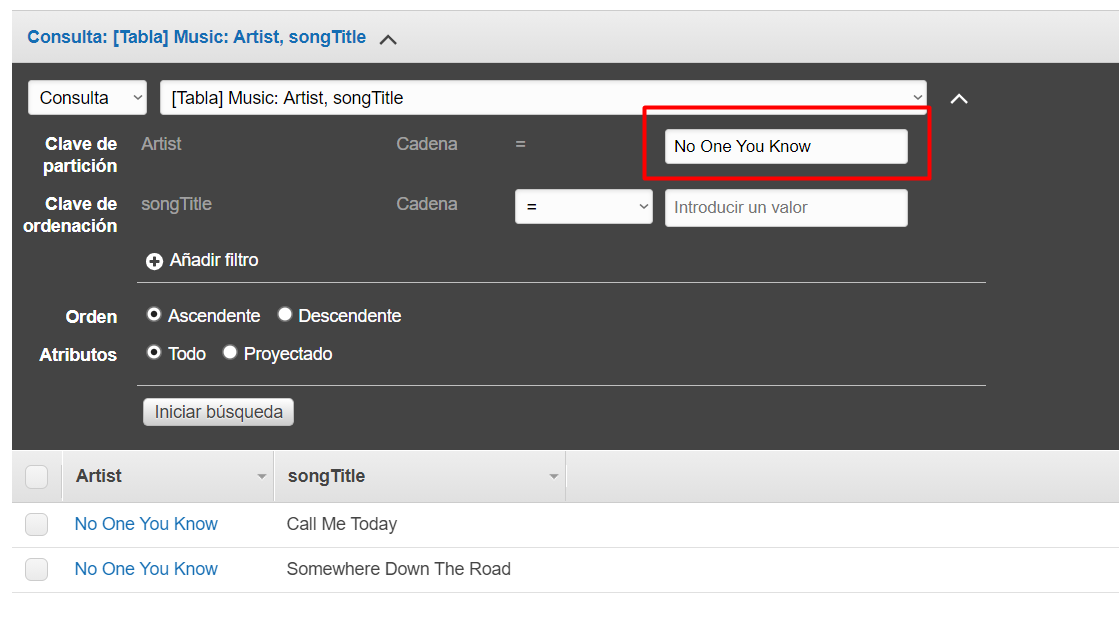
\includegraphics[width=15cm]{./images/11} 
	\end{center}
	\newpage
\textbf{3.3.Pruebe con otra consulta, pero esta vez acote los resultados de búsqueda:
}

    \begin{center}
		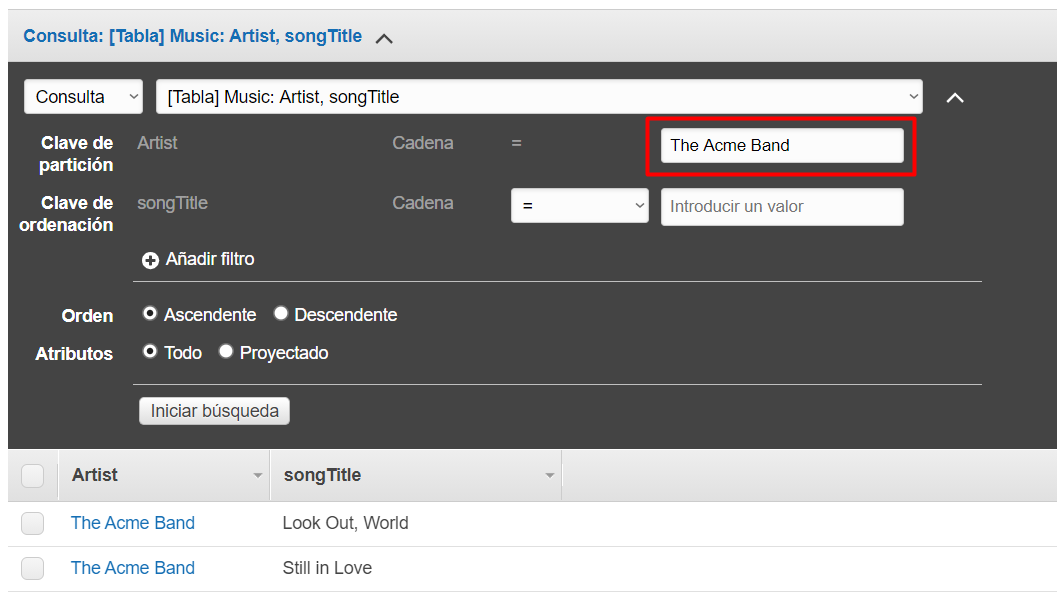
\includegraphics[width=15cm]{./images/12} 
	\end{center}
	\begin{center}
		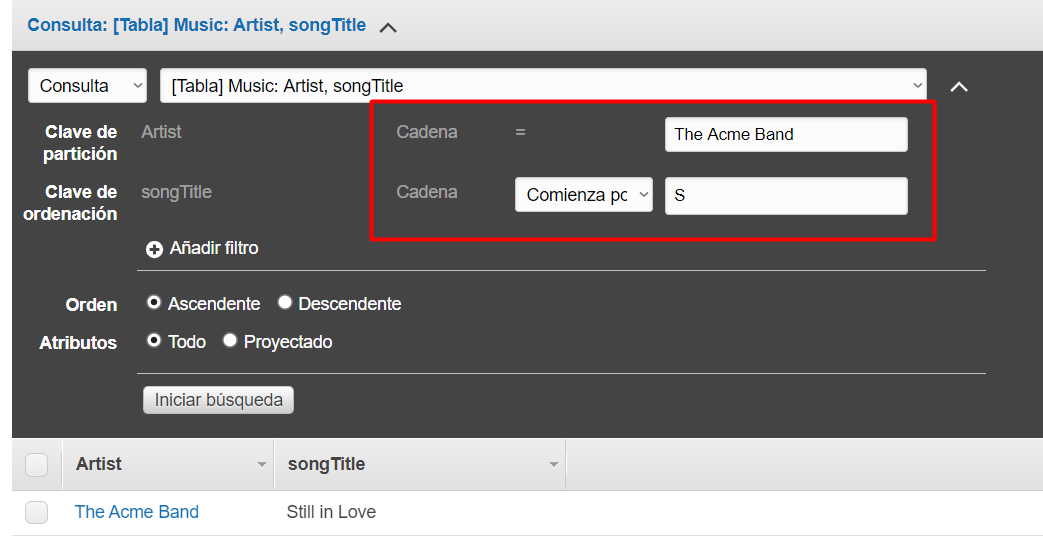
\includegraphics[width=15cm]{./images/13} 
	\end{center}

\newpage


\section{Eliminación de un elemento existente }

\textbf{4.1. Seleccione el desplegable Query (Consulta) para que vuelva a aparecer Scan (Escaneo).   }

    \begin{center}
		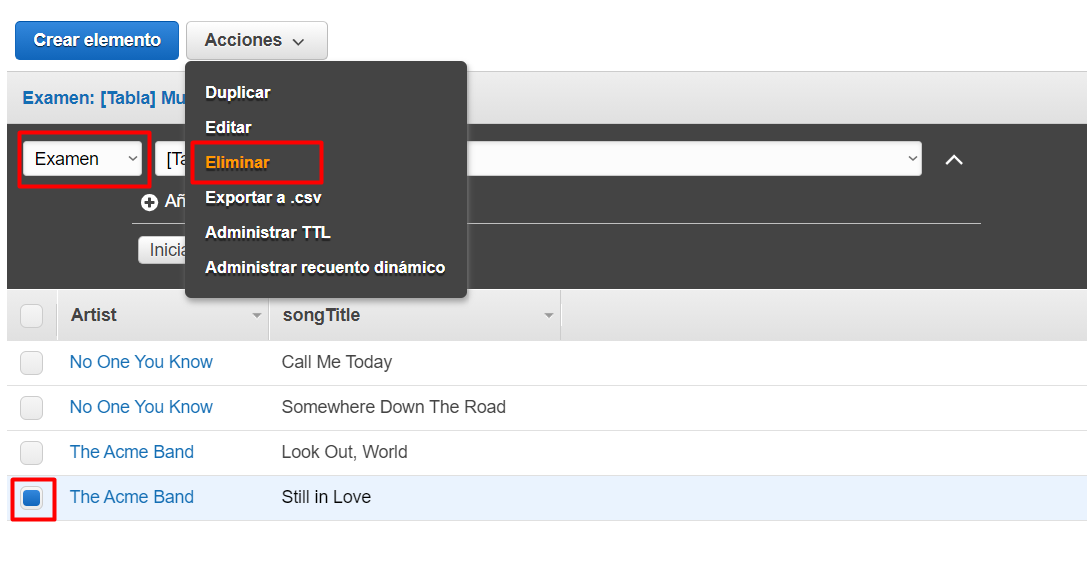
\includegraphics[width=15cm]{./images/14} 
	\end{center}

\newpage

\section{Eliminación de una tabla NoSQL }

\textbf{5.1. Puede eliminar con facilidad una tabla de la consola Amazon DynamoDB. Se recomienda eliminar las tablas que ya no utilice para que no le sigan cobrando por ellas. }
 \begin{center}
		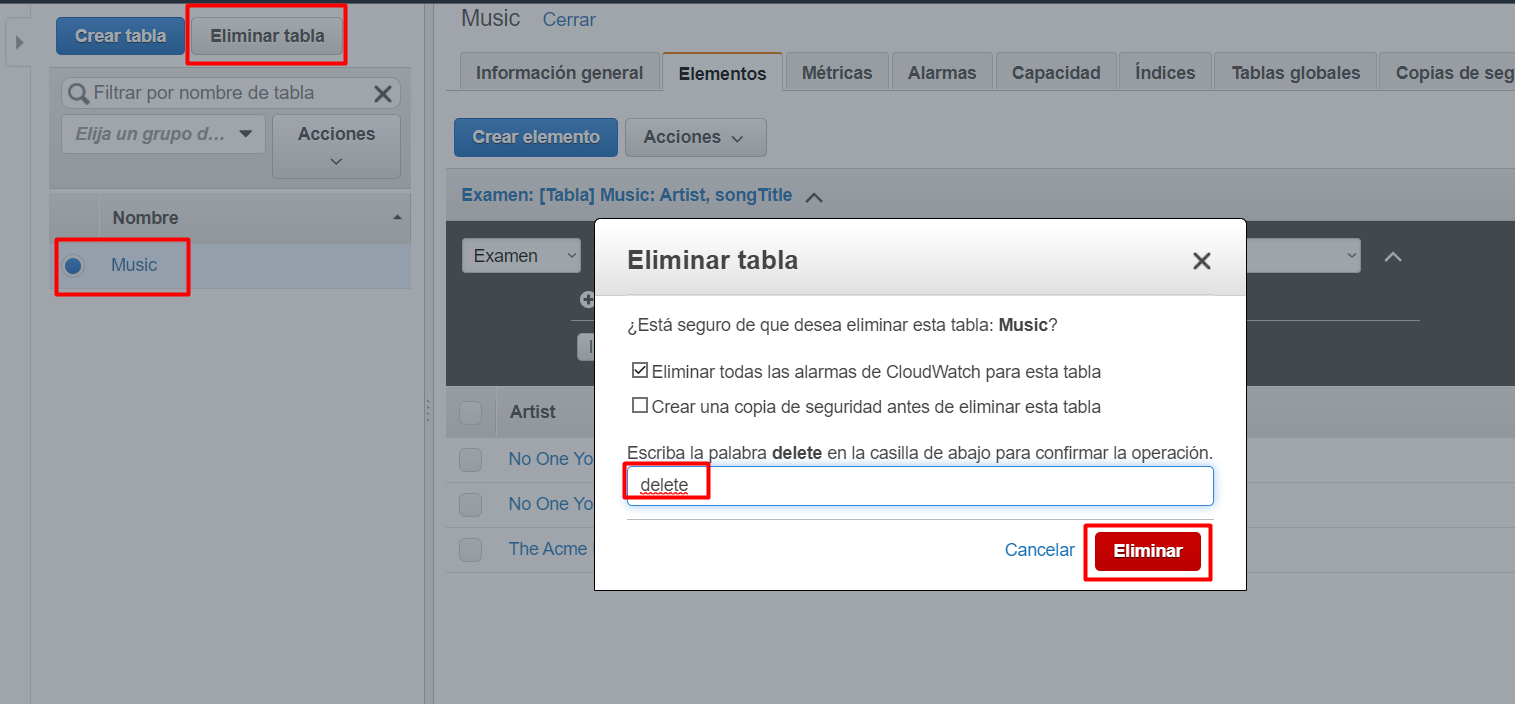
\includegraphics[width=15cm]{./images/15} 
	\end{center}
 \begin{center}
		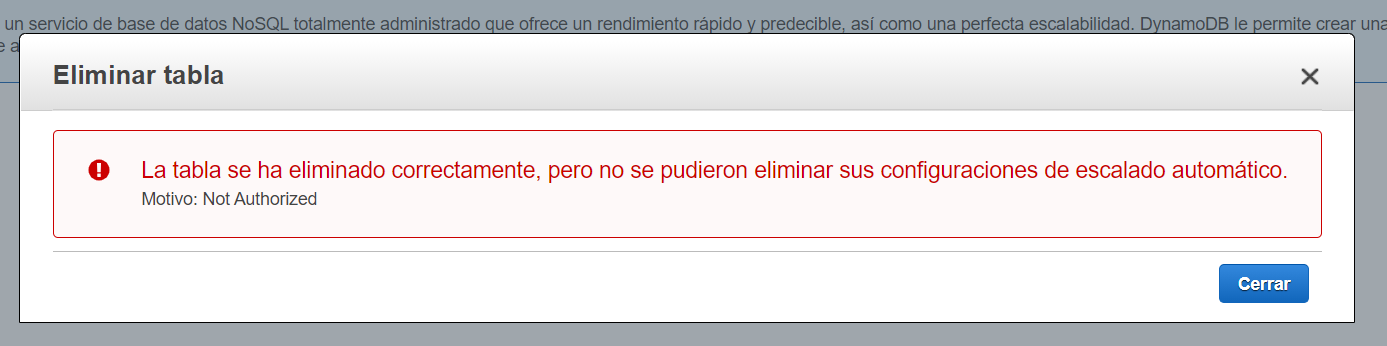
\includegraphics[width=15cm]{./images/16} 
	\end{center}


\end{document}